\documentclass[aps,prd,preprint,nofootinbib,11pt]{revtex4-2}
\usepackage{amsmath,amssymb,graphicx,booktabs,hyperref}
\newcommand{\R}{\mathbb R}
\begin{document}
\title{Spectral identifiability in a finite Planck bandpass moment model}
\author{Research supplement}
\noaffiliation
\date{October 25, 2026}
\begin{abstract}
We report a finite-table spectral identifiability calculation for seven nominal Planck frequency responses. The foreground family consists of five first-order synchrotron and dust moment columns, extended to nine columns at second order. Across six prescribed response conventions, the first-order matrices have numerically resolved rank five and admit a CMB-preserving foreground quotient. The second-order matrices have numerically resolved full row rank seven and admit explicit CMB degeneracy witnesses. Under the stipulated common spatial response, these statements apply to every coordinate of the signed low-multipole polarization tensor. The result concerns a linear model with independently varying signed moment amplitudes. No observed sky, noise covariance, null distribution, or physical truncation-error bound enters the calculation.
\end{abstract}
\maketitle
\renewcommand{\baselinestretch}{1.1}\selectfont
\section{Question and scope}
A frequency combination can preserve a calibrated CMB spectrum while removing a declared foreground subspace only if the CMB response lies outside that subspace. Counting frequency channels and foreground columns does not settle the question. Their actual spectral dependence matters. We therefore use released nominal bandpass tables to evaluate two explicit finite moment families, rather than assuming their ranks from their dimensions.

The calculation isolates a conditional question: would a common spatial response suffice for spectral separation in the chosen linear family? Moment expansions provide the physical motivation \cite{cmilc}; the finite family used here permits free signed moment amplitudes in every retained tensor coordinate. It is a relaxation of a truncated physical expansion. We do not require that every allowed amplitude array be realized by a nonlinear foreground law.

The associated numerical source contains the complete response matrices, column scales, singular spectra, quotient weights, degeneracy coefficients, and coordinate-wise controls. The figures below summarize frequency operators only. No angular tensor was replaced by a scalar statistic.
\clearpage
\section{Released tables and the finite response definition}
We use the LFI R3.31 tables for nominal 30, 44, and 70 GHz channels and HFI R3.00 F100, F143, and F217 tables, together with the 353 GHz PSB353 table \cite{rimoL,rimoH}. The last channel is explicitly PSB353. HFI F100 is selected by extension index two; equality of the duplicate F100 data extension was checked. LFI frequencies are in GHz and HFI coordinates are inverse centimetres. The latter become frequencies through $\nu=100c\,\widetilde\nu$.

Let $B_\nu(T)$ be the Planck intensity and $b_\nu=\partial_TB_\nu(T_{\rm CMB})$. The dimensionless finite response is
\begin{equation}
 R_i[S]=\frac{\operatorname{trapz}(\tau_i S,\nu_i)}
 {\operatorname{trapz}(\tau_i b_\nu,\nu_i)}.\label{eq:response}
\end{equation}
Here trapz defines the model on the retained released nodes. It is not a continuous-bandpass error certificate. For LFI, the intensity response is $\tau_i=g_i(\nu_{{\rm ref},i}/\nu)^2$, where $g_i$ is the released transmission. This distinction follows the antenna-temperature convention \cite{lfiCal,color}. HFI uses its retained raw transmission. Only positive frequencies and unflagged HFI rows with transmission above the specified threshold are retained. Adjacent retained nodes are joined, including across removed intervals; no tails are filled or extrapolated.

The six branches cross two LFI conventions with three HFI thresholds, $10^{-7}$, $10^{-8}$, and $10^{-6}$. Convention A uses the literal released frequencies. Convention B adds half the mean frequency-bin width to each LFI table before evaluating every frequency-dependent term. This reproduces an older reader operation \cite{color} as a version-sensitivity diagnostic. The R3 headers already mention a frequency correction; the relation between that correction and the older operation is unresolved. Neither convention B nor the branch envelope is a calibrated instrumental uncertainty model.

The fixed pivots are $T_{\rm CMB}=2.7255\,{\rm K}$, $\beta_s=-3$, $\beta_d=1.5$, $T_d=20\,{\rm K}$, $\nu_s=30\,{\rm GHz}$, and $\nu_d=353\,{\rm GHz}$. With reference amplitudes in thermodynamic kelvin, the intensity laws are
\begin{align}
 S_s&=b_{\nu_s}(\nu/\nu_s)^{\beta_s+2},\\
 S_d&=b_{\nu_d}(\nu/\nu_d)^{\beta_d}
             B_\nu(T)/B_{\nu_d}(T).
\end{align}
These pivots and all selection rules were fixed before the ranks were evaluated.
\clearpage
\section{Moment spaces and the complete tensor}
Define $t=(T-T_d)/T_d$ at the fixed dust pivot. Applying Eq.~\eqref{eq:response} to each spectrum gives the ordered matrices
\begin{align}
 F_1&=R[S_s,S_{s,\beta_s},S_d,S_{d,\beta_d},S_{d,t}],\\
 F_2&=[F_1,R[S_{s,\beta_s\beta_s},S_{d,\beta_d\beta_d},
 S_{d,\beta_dt},S_{d,tt}]].
\end{align}
Taylor factorials are absorbed into freely varying moment amplitudes. In particular, $S_{d,tt}=T_d^2\partial_T^2S_d$; it is not the repeated logarithmic-temperature derivative. Independent high-precision differentiation checked the implemented derivatives.

Let $a=(1,\ldots,1)^T\in\R^7$ denote the nominal CMB response after the unity integration check. In the stipulated common spatial response model,
\begin{equation}
 Y=a s^T+F U,\qquad Y\in\R^{7\times24}.
\end{equation}
The target $s$ retains signed $E_{\ell m}$ and $B_{\ell m}$ coordinates at $\ell=2,3$. Within each multipole the real ordering uses $m=0$, $\sqrt2\operatorname{Re}$ and $-\sqrt2\operatorname{Im}$ coordinates. Both polarizations and both multipoles remain present.

With frequency-major stacking, the complete operators are
\begin{equation}
 A=a\otimes I_{24},\qquad B=F\otimes I_{24}.
\end{equation}
Write $P_F=I-FF^+$ and $P=P_F\otimes I_{24}$. The exact conditional identity is
\begin{equation}
 PA=(P_Fa)\otimes I_{24},\qquad
 \operatorname{rank}(PA)=
 \begin{cases}24,&P_Fa\ne0,\\0,&P_Fa=0.\end{cases}\label{eq:rank}
\end{equation}
A nonzero frequency vector has rank one; its tensor product with the identity has rank 24. This algebraic statement concerns the declared linear model and holds independently of how numerical rank is assessed.

When $P_Fa\ne0$, the weight
\begin{equation}
 w=\frac{P_Fa}{a^TP_Fa},\qquad H=w^T\otimes I_{24}
\end{equation}
obeys $HA=I_{24}$ and $HB=0$. If $Fc=a$, every $v\in\R^{24}$ instead has the ambiguity $\delta s=v$, $\delta u=-c\otimes v$, for which $A\delta s+B\delta u=0$. Thus the complete target fibre, including all signed coordinates, is retained in the degeneracy description. Unspecified nuisance constraints have not been set to zero.
\clearpage
\section{Numerical result and conditioning}
For rank diagnostics each nuisance column is normalized to unit Euclidean norm. Singular values at least $10^{-10}$ are resolved nonzero; values at most $10^{-12}$ are unresolved at the prescribed criterion. Values between these thresholds would require an unresolved numerical-rank decision. These rules do not prove exact physical rank deficiency. Figure~\ref{fig:spectra} shows every stored singular value.

Every branch yields a five-dimensional resolved first-order foreground space and an augmented CMB-plus-foreground rank of six. The corresponding quotient passes explicit identity and nuisance-annihilation controls on the complete tensor operators. Every second-order matrix has seven resolved singular values. Its stored nine-coefficient witness reconstructs the CMB frequency response, and all target-coordinate degeneracy controls pass. The two findings persist across all six prescribed finite models.

\begin{table}[h]
\caption{Stored branch diagnostics. The label is the LFI convention followed by the HFI transmission threshold. Ranks are numerically resolved ranks $r_1/r_2$. Conditions $\kappa_j$ use unit-column matrices. $d_j=\sin\theta_j$ is the CMB-subspace principal-angle sine; $n_w=\|w\|_2$. The last column is the largest stored relative full-tensor degeneracy residual across target basis coordinates. The machine-readable companion also retains the spectral reconstruction residual.}
\resizebox{\textwidth}{!}{\begin{tabular}{lrrrrrrr}\toprule
Branch & $r_1/r_2$ & $\kappa_1$ & $\kappa_2$ & $d_1$ & $d_2$ & $n_w$ & $\epsilon_{24}$\\\midrule
A/$10^{-07}$ & 5/7 & 21.941 & 390.349 & 0.038540 & 3.98e-16 & 9.80717 & 1.01e-14 \\ 
A/$10^{-08}$ & 5/7 & 21.941 & 390.347 & 0.038540 & 6.51e-16 & 9.80716 & 1.39e-14 \\ 
A/$10^{-06}$ & 5/7 & 21.942 & 390.354 & 0.038539 & 5.10e-16 & 9.80722 & 1.67e-15 \\ 
B/$10^{-07}$ & 5/7 & 21.963 & 391.820 & 0.038445 & 6.01e-16 & 9.83119 & 6.53e-15 \\ 
B/$10^{-08}$ & 5/7 & 21.963 & 391.819 & 0.038445 & 3.28e-16 & 9.83118 & 2.30e-15 \\ 
B/$10^{-06}$ & 5/7 & 21.963 & 391.826 & 0.038445 & 6.79e-16 & 9.83124 & 7.71e-15 \\ 

\end{tabular}}\label{tab:branches}
\end{table}
The first-order principal angle is small even though the quotient is resolved. The signed weights in Fig.~\ref{fig:weights} exhibit substantial cancellation. Their norm is a Euclidean amplification diagnostic. It is not a measured noise standard deviation, and the present metric is not an inverse noise covariance. Unit-column normalization changes singular-value conditioning but preserves the exact column space.

The accepted numerical evidence includes independently assembled responses at high precision, exact conversion of released source floats, direct derivative controls, CMB unity, nonzero column-rescaling invariance, nesting of the moment spaces, synthetic duplicate-column rank loss, and rejection of an injected CMB nuisance. The full coordinate controls are included in the source data. These implementation checks concern the specified finite calculation; synthetic controls supply no sky evidence.

Equation~\eqref{eq:rank} states an exact conditional alternative. The table supplies numerical support for the corresponding cases in these particular finite branches. We keep these two levels of assertion distinct.
\clearpage
\begin{figure}[h]
\centering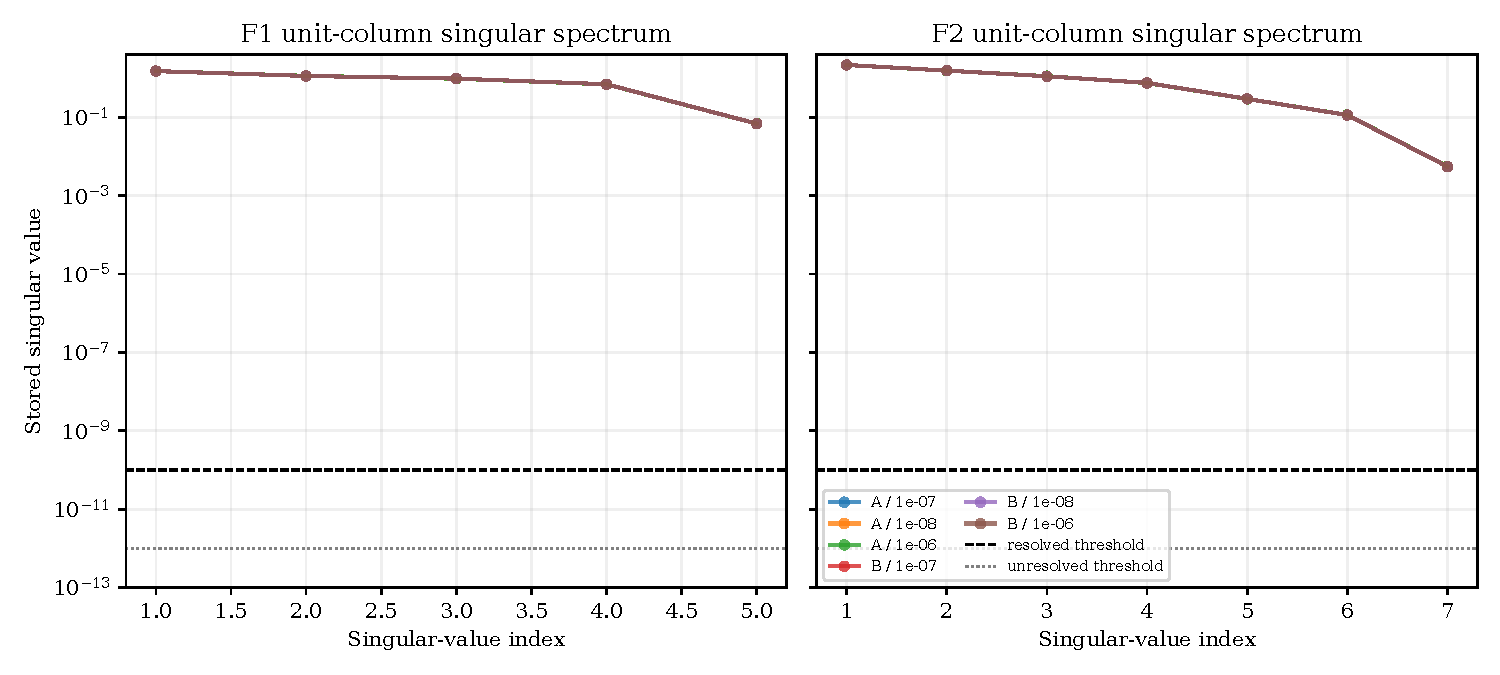
\includegraphics[width=\textwidth]{figures/spectra.pdf}
\caption{Complete normalized singular spectra for both moment matrices in all six branches. Dashed and dotted lines show the prescribed resolved and unresolved thresholds. Curves nearly coincide; all branches are plotted independently without averaging. The five first-order and seven second-order singular values are well above the resolved threshold. Values and thresholds come directly from the stored numerical result and its fixed definition. These are finite spectral-operator diagnostics under a common spatial response, with no observed-sky or noise calibration.}\label{fig:spectra}
\end{figure}
\section{What the obstruction means}
The second-order result blocks a universal CMB-preserving linear annihilator for the declared free signed moment family in each target coordinate. More channels than foreground components are not available in this model once the admitted columns span the channel space. A first-order quotient can therefore be an accurate implementation of an insufficient foreground model.

This does not establish a universal inability to separate CMB. Nonlinear physical relations, sign restrictions, priors connecting moment amplitudes, additional frequencies, or qualified spatial information could change the admissible family. None of those constraints has been imposed here. Likewise, the first-order quotient is conditional on the common spatial response and on the truncation itself. No remainder bound is available for omitted moments or spectral tails.

A blackbody-spectrum nuisance with the same operator as the target remains exactly confounded with it, independently of these synchrotron and dust calculations. Spectral annihilation alone cannot distinguish two contributions with identical responses.
\clearpage
\begin{figure}[h]
\centering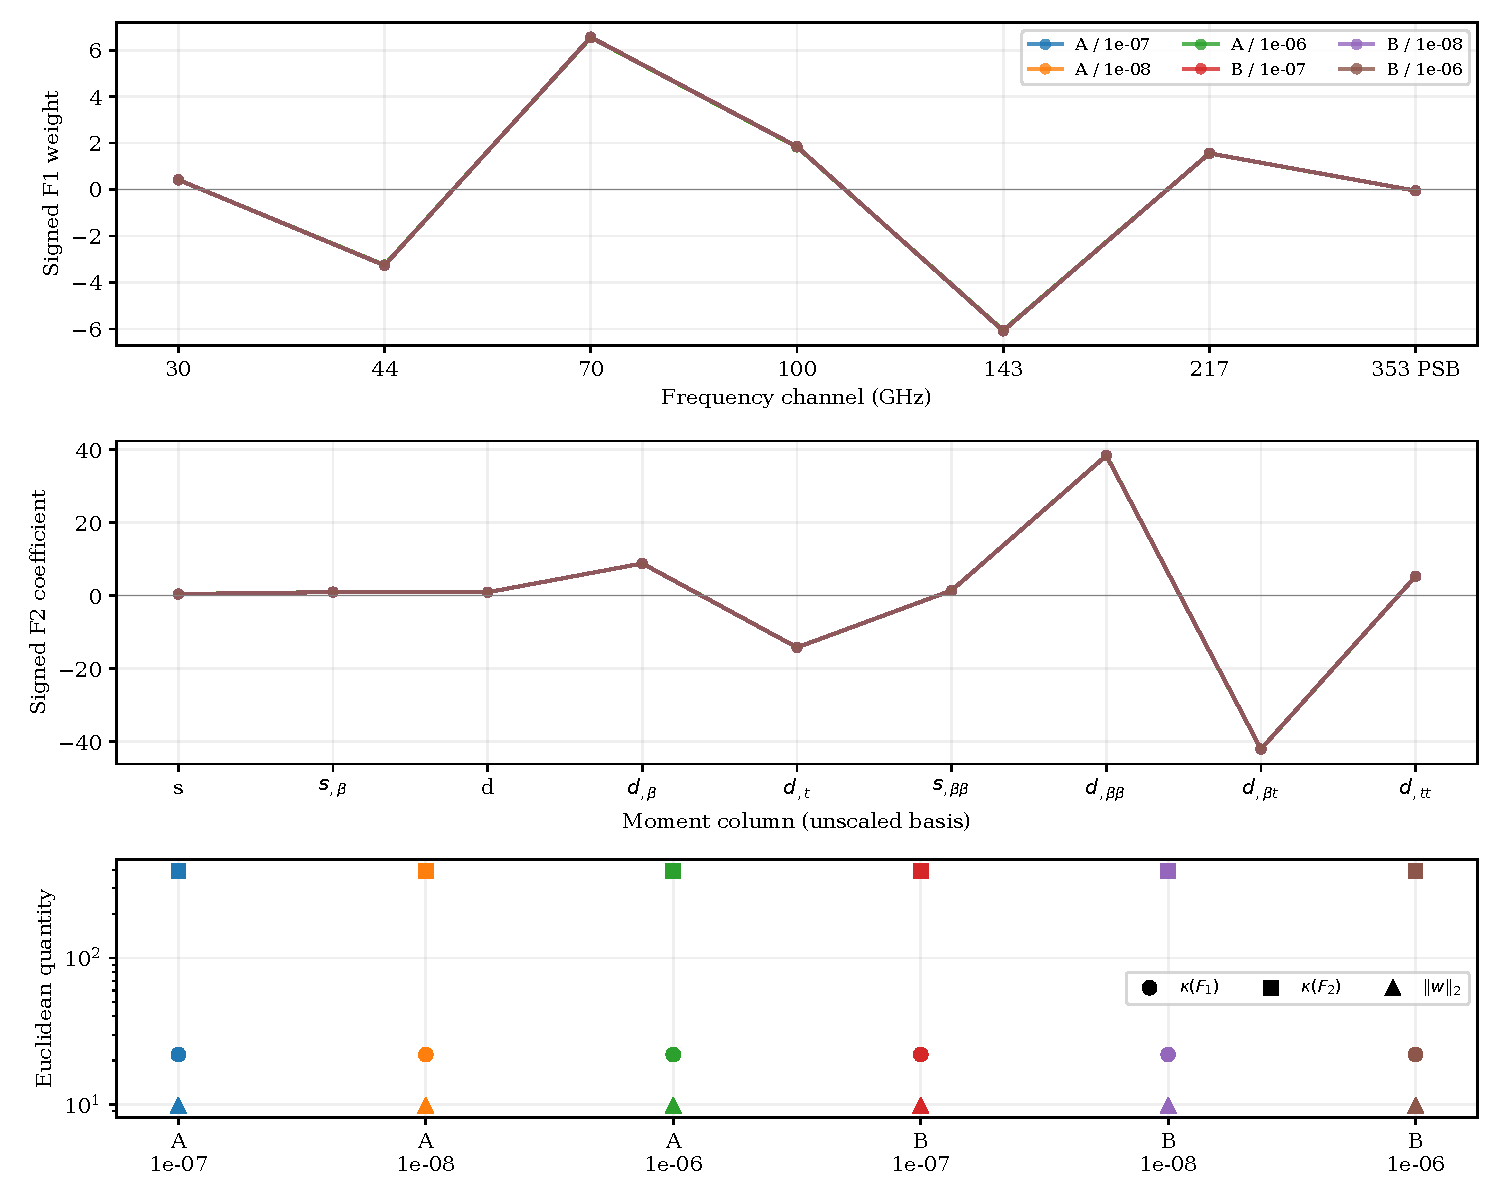
\includegraphics[width=.96\textwidth,height=.72\textheight,keepaspectratio]{figures/weights_witnesses.pdf}
\caption{All stored signed first-order quotient weights (top), all nine signed second-order CMB-reconstruction coefficients in the unscaled moment basis (middle), and their conditioning diagnostics (bottom), for every branch. The second-order coefficients satisfy $F_2c\simeq a$; the full-tensor degeneracy uses $-c\otimes v$, so its nuisance shift has the opposite sign. Circles and squares in the lower panel denote unit-column condition numbers; triangles denote the first-order weight norm. Nearly coincident curves remain separately represented. These quantities describe the stipulated finite linear family and do not estimate instrumental noise.}\label{fig:weights}
\end{figure}
\clearpage
\section{Limits and reproducibility}
A nominal average passband does not establish a common component-specific polarized map response \cite{planckIV}. Polarization efficiency, angle calibration, beam and scan coupling, mapmaking, and angular truncation can enter the actual response. QuickPol illustrates the need to retain polarized beam coupling when describing instrumental effects \cite{quickpol}. None of those effects is inferred from the temperature-normalization denominator in Eq.~\eqref{eq:response}.

No observed quotient tensor or physical amplitude $x$ has been measured. The physical filling fraction is not evaluable, $Q$ has not been evaluated, $\Pi$ has not been calibrated, and $G_F$ is inapplicable because frequency is not depth. The foreground matrix $F_j$ in this supplement is a spectral design matrix, not a physical filling fraction. There is no likelihood, posterior, null probability, or geometry classification in the result.

Application to an observed sky would require a source-qualified component-dependent spatial and spectral response, a declared angular domain, control of omitted-domain and omitted-moment terms, and a justified joint residual or noise model. Numerical rank at nominal response does not imply uniform identifiability over response uncertainty. The six finite branches do not replace such an uncertainty model.

The companion source archive contains the full accepted numerical result and independent check, including all coordinate residuals, as well as the figure-generation script and generated branch table. The script reads stored fields only; it performs no integration, decomposition, or fit. The archive builds the figures and this supplement locally. Detailed source identities and scientific qualification are retained alongside it. Reproducing the original spectral calculation requires the separately identified released tables and prescribed numerical procedure; compiling the supplement requires neither a map download nor a scientific rerun.

The finite result is consequently specific and useful: first-order spectral cancellation remains possible in every prescribed branch, whereas the admitted second-order linear family spans the complete target response. Its relevance to data depends on whether the physical response and foreground domain justify one of those families.
\bibliographystyle{apsrev4-2}
\bibliography{references}
\end{document}
